\chapter{UAV Navigation Using the RBL Algorithm and LiDAR Sensing\label{chap:lidar}}

    \section{Introduction}
        \subsection{Motivation}
        \ac{UAV}s are increasingly being deployed in challenging, unstructured environments like dense forests, moving beyond their traditional use in open areas.
        This shift is driven by a growing demand for autonomous solutions in sectors like environmental monitoring, forestry management (health assessment \cite{kurovec_fel_clanek}), and search and rescue, where ground-based access is difficult. 
        Furthermore, this work aligns with the broader trend of deploying \ac{UAV}s for increasingly complex tasks, such as detailed infrastructure inspection (e.g., power lines, where autonomous navigation in cluttered, potentially high \ac{EMI} environments is essential (Fly4Future \cite{f4f_powerline_inspection})). 
        Enabling UAVs to reliably navigate point-to-point within these challenging settings is a foundational step towards realizing these advanced applications safely and efficiently.

        While the primary objective of this work is to enable successful point-to-point navigation within a forest using the \ac{RBL} algorithm, a significant secondary benefit emerges from this process. 
        By successfully navigating from point A to point B while simultaneously building a map of the traversed environment, the UAV generates valuable spatial data about the forest structure. 
        This autonomously generated map can then serve a vital purpose: enabling enhanced planning for future missions within the same area. 
        Once a map exists, subsequent UAV operations could potentially transition from purely reactive navigation strategies to more efficient, globally informed path planning algorithms such as TODO find some. 
        Leveraging prior knowledge of obstacle locations could significantly improve the safety and efficiency of future routine tasks.
        
        \subsection{Problem Statement}
            Operating UAVs effectively within complex, three-dimensional environments like forests presents significant navigational challenges that hinder widespread autonomous deployment. 
            The primary problems addressed in this work stem from:
            \begin{enumerate}
                \item \textbf{\ac{GNSS}-Denied Conditions: } \\
                Within forests, the dense canopy and other obstructions frequently block or scatter \ac{GNSS} signals, leading to unreliable or completely absent reception.
                This necessitates reliance on onboard sensors and algorithms (like \ac{SLAM} based on \ac{LiDAR} and \ac{IMU} data) for accurate localization and state estimation.
                \item \textbf{Cluttered and Unpredictable Environments: } \\
                Forests are inherently cluttered with numerous static obstacles (trees, trunks, branches) and potentially dynamic ones (animals, leafs, falling branches). 
                The navigation system must be capable of perceiving these obstacles in real-time and planning safe paths around them without prior knowledge of their exact layout.
            \end{enumerate}
            Therefore, the core problem is to develop and validate a robust autonomous navigation system that allows a UAV to reliably traverse between specified points in a cluttered, GNSS-denied forest environment using only onboard sensing and computation.

        \subsection{Objectives}
            The primary objectives within this chapter are: 
            \begin{itemize}
                \item \textbf{Integrate the \ac{RBL} with Onboard Sensing: } \\
                    Adapt the core of the \ac{RBL} to utilize real-time sensor data. 
                    This includes modification of sensing cell $\mathcal{S}$, because used \ac{LiDAR} doesnt see in all directions. 
                    Sensing cell needs to remain convex so the centroid computed from partitioned cell $\mathcal{A}$ is never computed outside of the set - for safety convergence towards the goal.
                \item \textbf{Process Point Cloud Data: } \\
                    Implement neccessary filtration to refine the raw point cloud data acquired from the \ac{LiDAR}.
                \item \textbf{Integrate external packages on the \ac{UAV}: } \\
                    Integrate and configure external software packages for simultaneous environmental mapping and robust state estimation, suitable for operation within the \ac{GNSS}-denied forest environment.
                \item \textbf{Experimental Validation: } \\
                    Conduct experiments to evaluate the performance, robustness, and effectiveness of the complete navigation solution. 
                    This validation will be performed through real-world flight tests in an actual forest.
            \end{itemize}

        \subsection{Chapter Overview}
            TODO Summary of what this chapter covers

    \section{LiDAR-Based Perception and Point Cloud Processing}
        \subsection{Overview of LiDAR for UAV Navigation}
            \ac{LiDAR} is a crucial sensing technology widely used in applications such as SLAM \cite{pointlio_mrs}, autonomous vehicles \cite{Lidar_autonomous_vehicles}, UAVs TODOcite, and precision agriculture \cite{Lidar_agriculture}. 
            It provides high-resolution spatial data about the surrounding environment, making it a valuable tool for perception and navigation in dynamic and complex environments.  
            For UAV applications, \ac{LiDAR} serves several essential functions:  
            \begin{itemize}  
                \item \textbf{3D Mapping} -- Capturing a detailed representation of terrain, structures, and obstacles.  
                \item \textbf{Obstacle Detection} -- Identifying objects and estimating their position relative to the \ac{UAV} for collision avoidance.  
                \item \textbf{Autonomous Path Planning} -- Assisting navigation algorithms by providing spatial information for decision-making.  
                \item \textbf{Terrain Following} -- Helping the \ac{UAV} maintain a safe altitude by detecting variations in ground elevation.  
            \end{itemize}  

            \ac{LiDAR} offers several benefits that make it an attractive choice for \ac{UAV}-based navigation:  
            \begin{itemize}  
                \item \textbf{High Accuracy} -- Provides precise distance measurements, crucial for obstacle avoidance and localization.  
                \item \textbf{Environment Agnostic} -- Functions effectively in various conditions, including low-light environments and featureless terrain where cameras may fail.  
                \item \textbf{Fast Data Acquisition} -- Captures thousands to millions of points per second, enabling real-time processing.  
                \item \textbf{Rich Depth Information} -- Unlike cameras that provide only 2D images, \ac{LiDAR} generates accurate depth data, improving spatial awareness and 3D perception.  
            \end{itemize}  

            Despite its advantages, \ac{LiDAR} also presents certain challenges and limitations:  
            \begin{itemize}  
                \item \textbf{Computational Complexity} -- Processing large point clouds in real-time requires significant computational power, which may be a limitation for \ac{UAV}s with low processing resources.
                \item \textbf{Sensor Noise and Artifacts} -- External factors such as vibrations and motion of \ac{UAV} can introduce errors in point cloud data.  
                \item \textbf{Limited Field of View (FoV)} -- The placement of the \ac{LiDAR} sensor on the \ac{UAV} affects its coverage, requiring strategies to compensate for blind spots.  
                \item \textbf{Environmental Interference} -- Performance may degrade in challenging conditions such as fog, rain, or dense vegetation due light deviation.  
                \item \textbf{Power Consumption} -- \ac{LiDAR} sensors can consume a significant amount of power, which reduces the overall flight time of the \ac{UAV}.
                \item \textbf{Interference with Other LiDARs} -- \ac{LiDAR} sensors can experience interference when multiple units are used nearby, potentially leading to faulty measurements.
            \end{itemize}

        \subsection{Point Cloud Data Acquisition}
            \ac{LiDAR} systems determine object distances by emitting laser pulses and measuring the time it takes for the reflected light to return. 
            This process, known as \ac{ToF}, involves scanning the environment with laser beams directed at varying horizontal and vertical angles. 
            The reflected light, modulated in intensity, phase, or frequency, is captured by a receiver, which uses a lens to focus the signal onto a photodetector. 
            This detector converts the light into an electrical signal via the photoelectric effect \cite{lidar_how_works}.

            The system calculates distance based on the light's travel time, considering its near-light-speed propagation. 
            To distinguish transmitted from received signals, the laser's \setcounter{tocdepth}{1}
            wavelength is often adjusted. 
            Subsequent signal processing filters and analyzes the electrical signal, accounting for surface material and environmental variations. 
            The output is a 3D point cloud representing the scanned environment, along with reflected laser energy intensities. 
            All these data points are stored in a ROS message of type \(sensor\_msgs::PointCloud2\)

        \subsection{Preprocessing Techniques}
            To efficiently process \ac{LiDAR} data and reduce computational complexity, the raw point cloud undergoes downsampling and filtering. 
            The point cloud density is reduced using a voxel grid filter. 
            Subsequently, points associated with the \ac{UAV}'s structure are removed based on its known encumbrance.
            \begin{itemize}
                \item \textbf{Voxel Grid Downsampling} -- The raw \ac{LiDAR} point cloud often contains a large number of points, which can be computationally expensive to process in real-time. 
                To address this, we apply a voxel grid filter using the \ac{PCL} \cite{pcl_voxelgrid}. 
                This method partitions the 3D space into a grid of voxels with a given resolution (leafSize) and retains a single representative point per voxel. 
                The filtering process reduces the number of points while preserving the overall structure of the environment.
                \item \textbf{Filtering Points Corresponding to the UAV Structure} -- \ac{LiDAR} sensors mounted on \ac{UAV}s can capture unwanted points originating from the \ac{UAV} itself, such as reflections from its frame or rotor rods. 
                To prevent these points from interfering with navigation, additional filtering step has been applied.
                Points falling outside a specified distance range (closer than a minimum threshold or farther than a maximum threshold) are filtered out.
            \end{itemize}
            The resulting filtered point cloud contains only relevant environmental features while eliminating unnecessary points, improving efficiency for future processes.
            The point cloud is than fed into Point lio state estimator and bonxai mapping. TODO get access to repo.

        \subsection{Bonxai Mapping}
            As will be shown later in this chapter, prior terrain knowledge is beneficial for navigation. 
            For this purpose, environmental mapping was accomplished using a simple package developed by the MRS group, implementing the Bonxai mapping approach.
            The resulting map is represented as a voxel grid, which is then used by the \ac{RBL} algorithm for navigation planning.

            Initially, an approach involving surface reconstruction from this voxel data was investigated. 
            This involved estimating surface normals from the point cloud combined with Greedy Projection Triangulation (GP3) method from the PCL library to generate polygonal mesh approximating the environment's surface.
            While this method could produce relatively accurate surface representation, it turned out to be computationally expensive and too slow for real-time execution on the \ac{UAV}'s onboard computer.

            Due to these limitations, the surface reconstruction approach was abandoned. 
            Instead a simpler and more efficient method was adopted, which involves directly using the information about the environment stored in voxel grid map.
            This direct voxel usage approach is detailed in the subsequent section. 
            Consequently, further development of the mesh-based surface reconstruction method is not recommended for this application.

            \begin{figure}[H]
                \centering
                \subfloat[Surface approximation using Greedy Projection Triangulation] {
                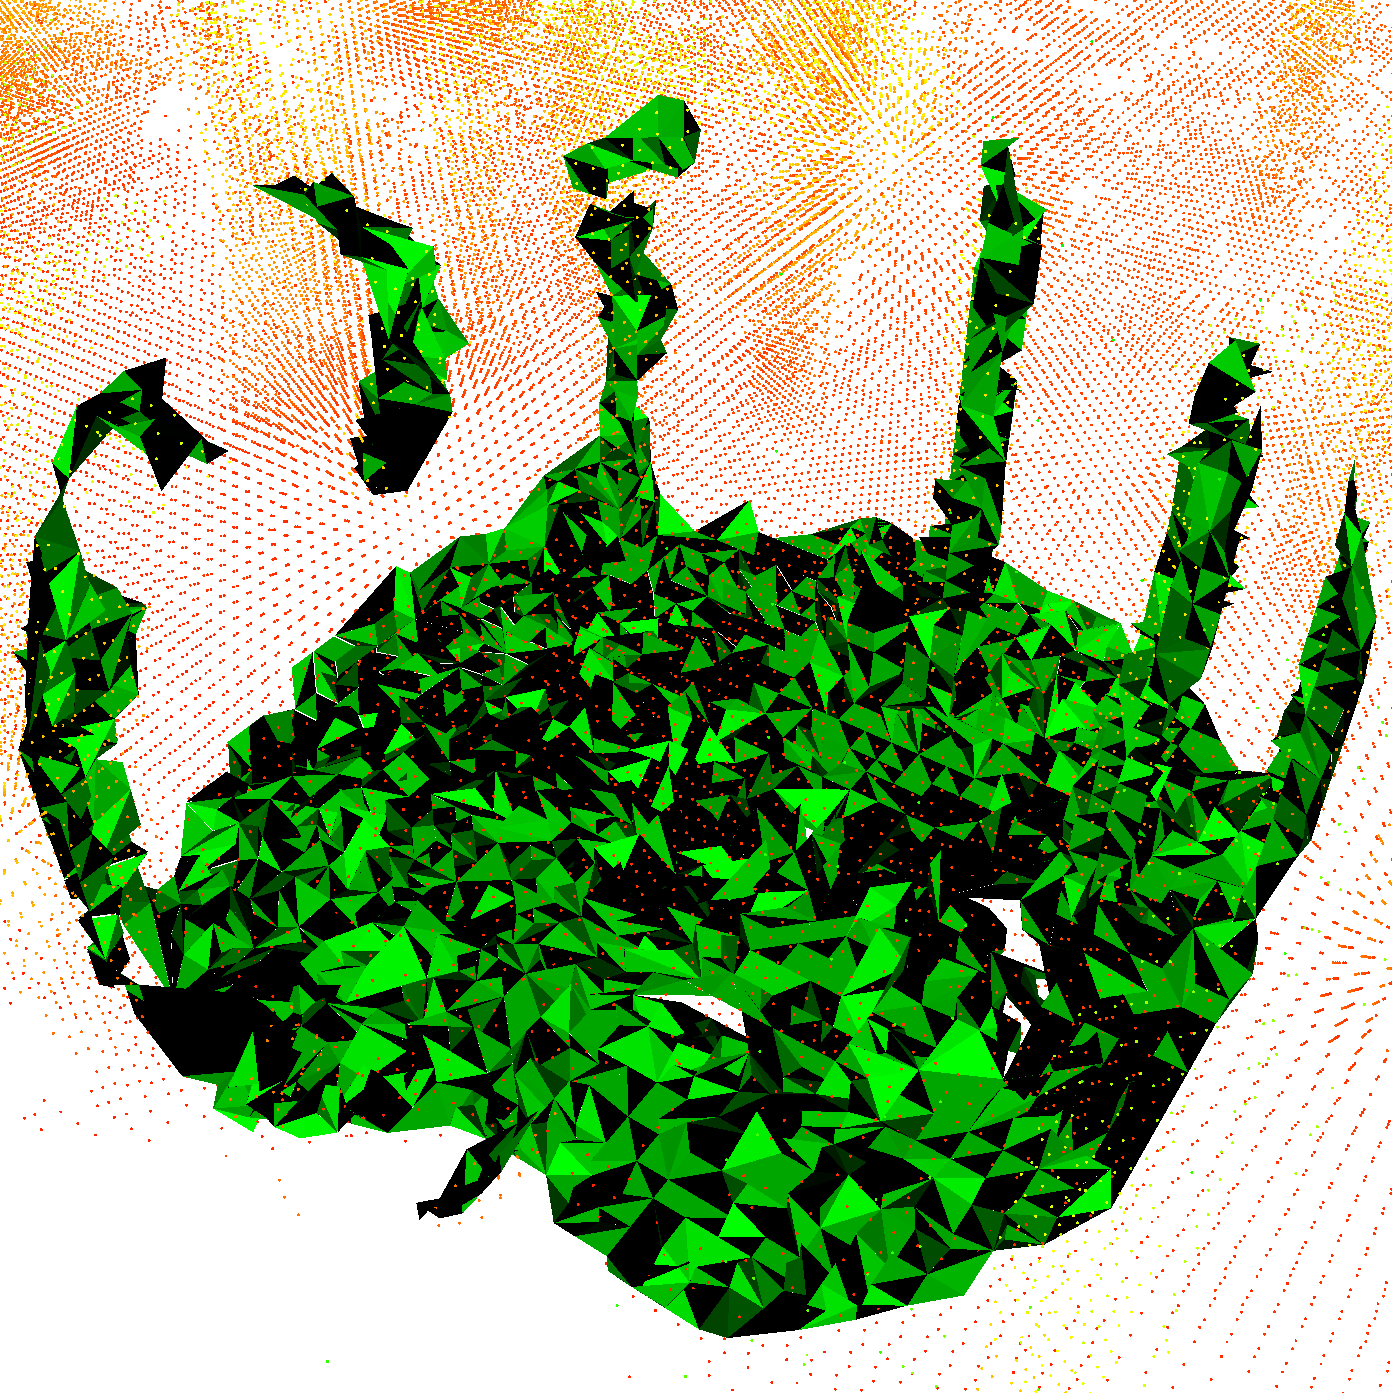
\includegraphics[width=0.48\textwidth]{./fig/rviz/triangulation_surface_aprox.png}
                \label{fig:triangulation_fig}
                }
                \caption{
                    Surface approximation using Greedy Projection Triangulation.
                }
                \label{fig:triangulation}
            \end{figure}

        \subsection{Voxel-Based Modification of Cell $\mathcal{A}$}
            Given that the size of the voxels is known, this infromation can be used to refine the partitioning of cell $\mathcal{A}$ by treating voxels as obstacles.
            First, it is necessary to determine which voxels are relevant to the \ac{RBL} algorithm.
            This can be achieved by considering the scaling parameter $\eta$.
            A voxel is considered relevant if it lies within radius of $\frac{r_s}{\eta}$ of the agent.
            For each discrete point in  in the set composing cell $\mathcal{S}$, the nearest voxel is identified using k-d tree algorithm from the PCL library.
            Because the found point is the voxel's center, the closest pint within that voxel's boundaries is calculated to accurate partition the cell $\mathcal{A}$ from cell $\mathcal{S}$.

            Given a point $\mathbf{p_{\mathcal{S}}}$, the voxel center $\mathbf{v_c}$ and the voxel edge length $\mathbf{e}$, $\mathbf{p_{closest}}$, is computed as: 
            \begin{equation}
                \mathbf{p}_{closest} =
                \begin{pmatrix}
                    \text{clamp}(p{\mathcal{S},x}, v_{c,x} - \frac{\mathbf{e}}{2}, v_{c,x} + \frac{\mathbf{e}}{2}) \\
                    \text{clamp}(p_{\mathcal{S},y}, v_{c,y} - \frac{\mathbf{e}}{2}, v_{c,y} + \frac{\mathbf{e}}{2}) \\
                    \text{clamp}(p_{\mathcal{S},z}, v_{c,z} - \frac{\mathbf{e}}{2}, v_{c,z} + \frac{\mathbf{e}}{2})
                \end{pmatrix}
            \end{equation}
            where function clamp(x, a, b) constrains the value x to the range [a, b].
            This constrains $\mathbf{p_{\mathcal{S}}}$ to the voxel boundaries.

            A point is excluded from the set if $ \| \mathbf{p_i} - \mathbf{p_{\mathcal{S}}} \| \leq \eta \cdot \| \mathbf{p_i} - \mathbf{p}_{closest}\|$.
            

    \section{Implementation and Integration on UAV}
        \subsection{Challanges in Integration}
            The algorithm's performance is influenced by the limitations of the \ac{LiDAR} sensor used for environmental sensing. 
            While the algorithm functions optimally with a full 360° horizontal and 180° vertical \ac{FOV}, which would require multiple sensors, the experiments used a single Livox Mid 360 \ac{LiDAR} \cite{livox_mid360}. 
            This \ac{LiDAR} provides a 360° horizontal \ac{FOV} and only a 59° vertical \ac{FOV}, resulting in a sensing blind spot.

            To solve this limitation, several modification were implemented. 
            The \ac{LiDAR} was mounted at an angle $\gamma$, as shown in Figure \reffig{fig:uavs}, to enhance ground sensing and increase forward visibility.

            \begin{figure}[htbp]
                \centering
                \subfloat[UAV model with visualized \ac{LiDAR} mounting parameters.] {
                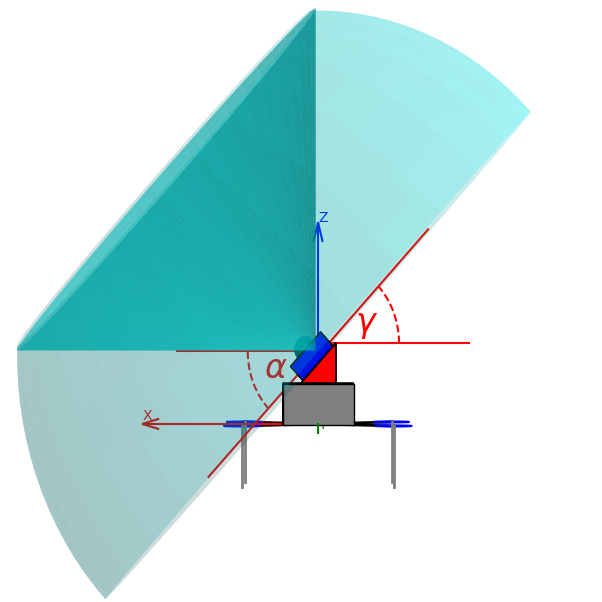
\includegraphics[width=0.48\textwidth]{./fig/photos/uav_side_view.png}
                \label{fig:model_uav}
                }
                \subfloat[UAV used in the experiment with mounted \ac{LiDAR}] {
                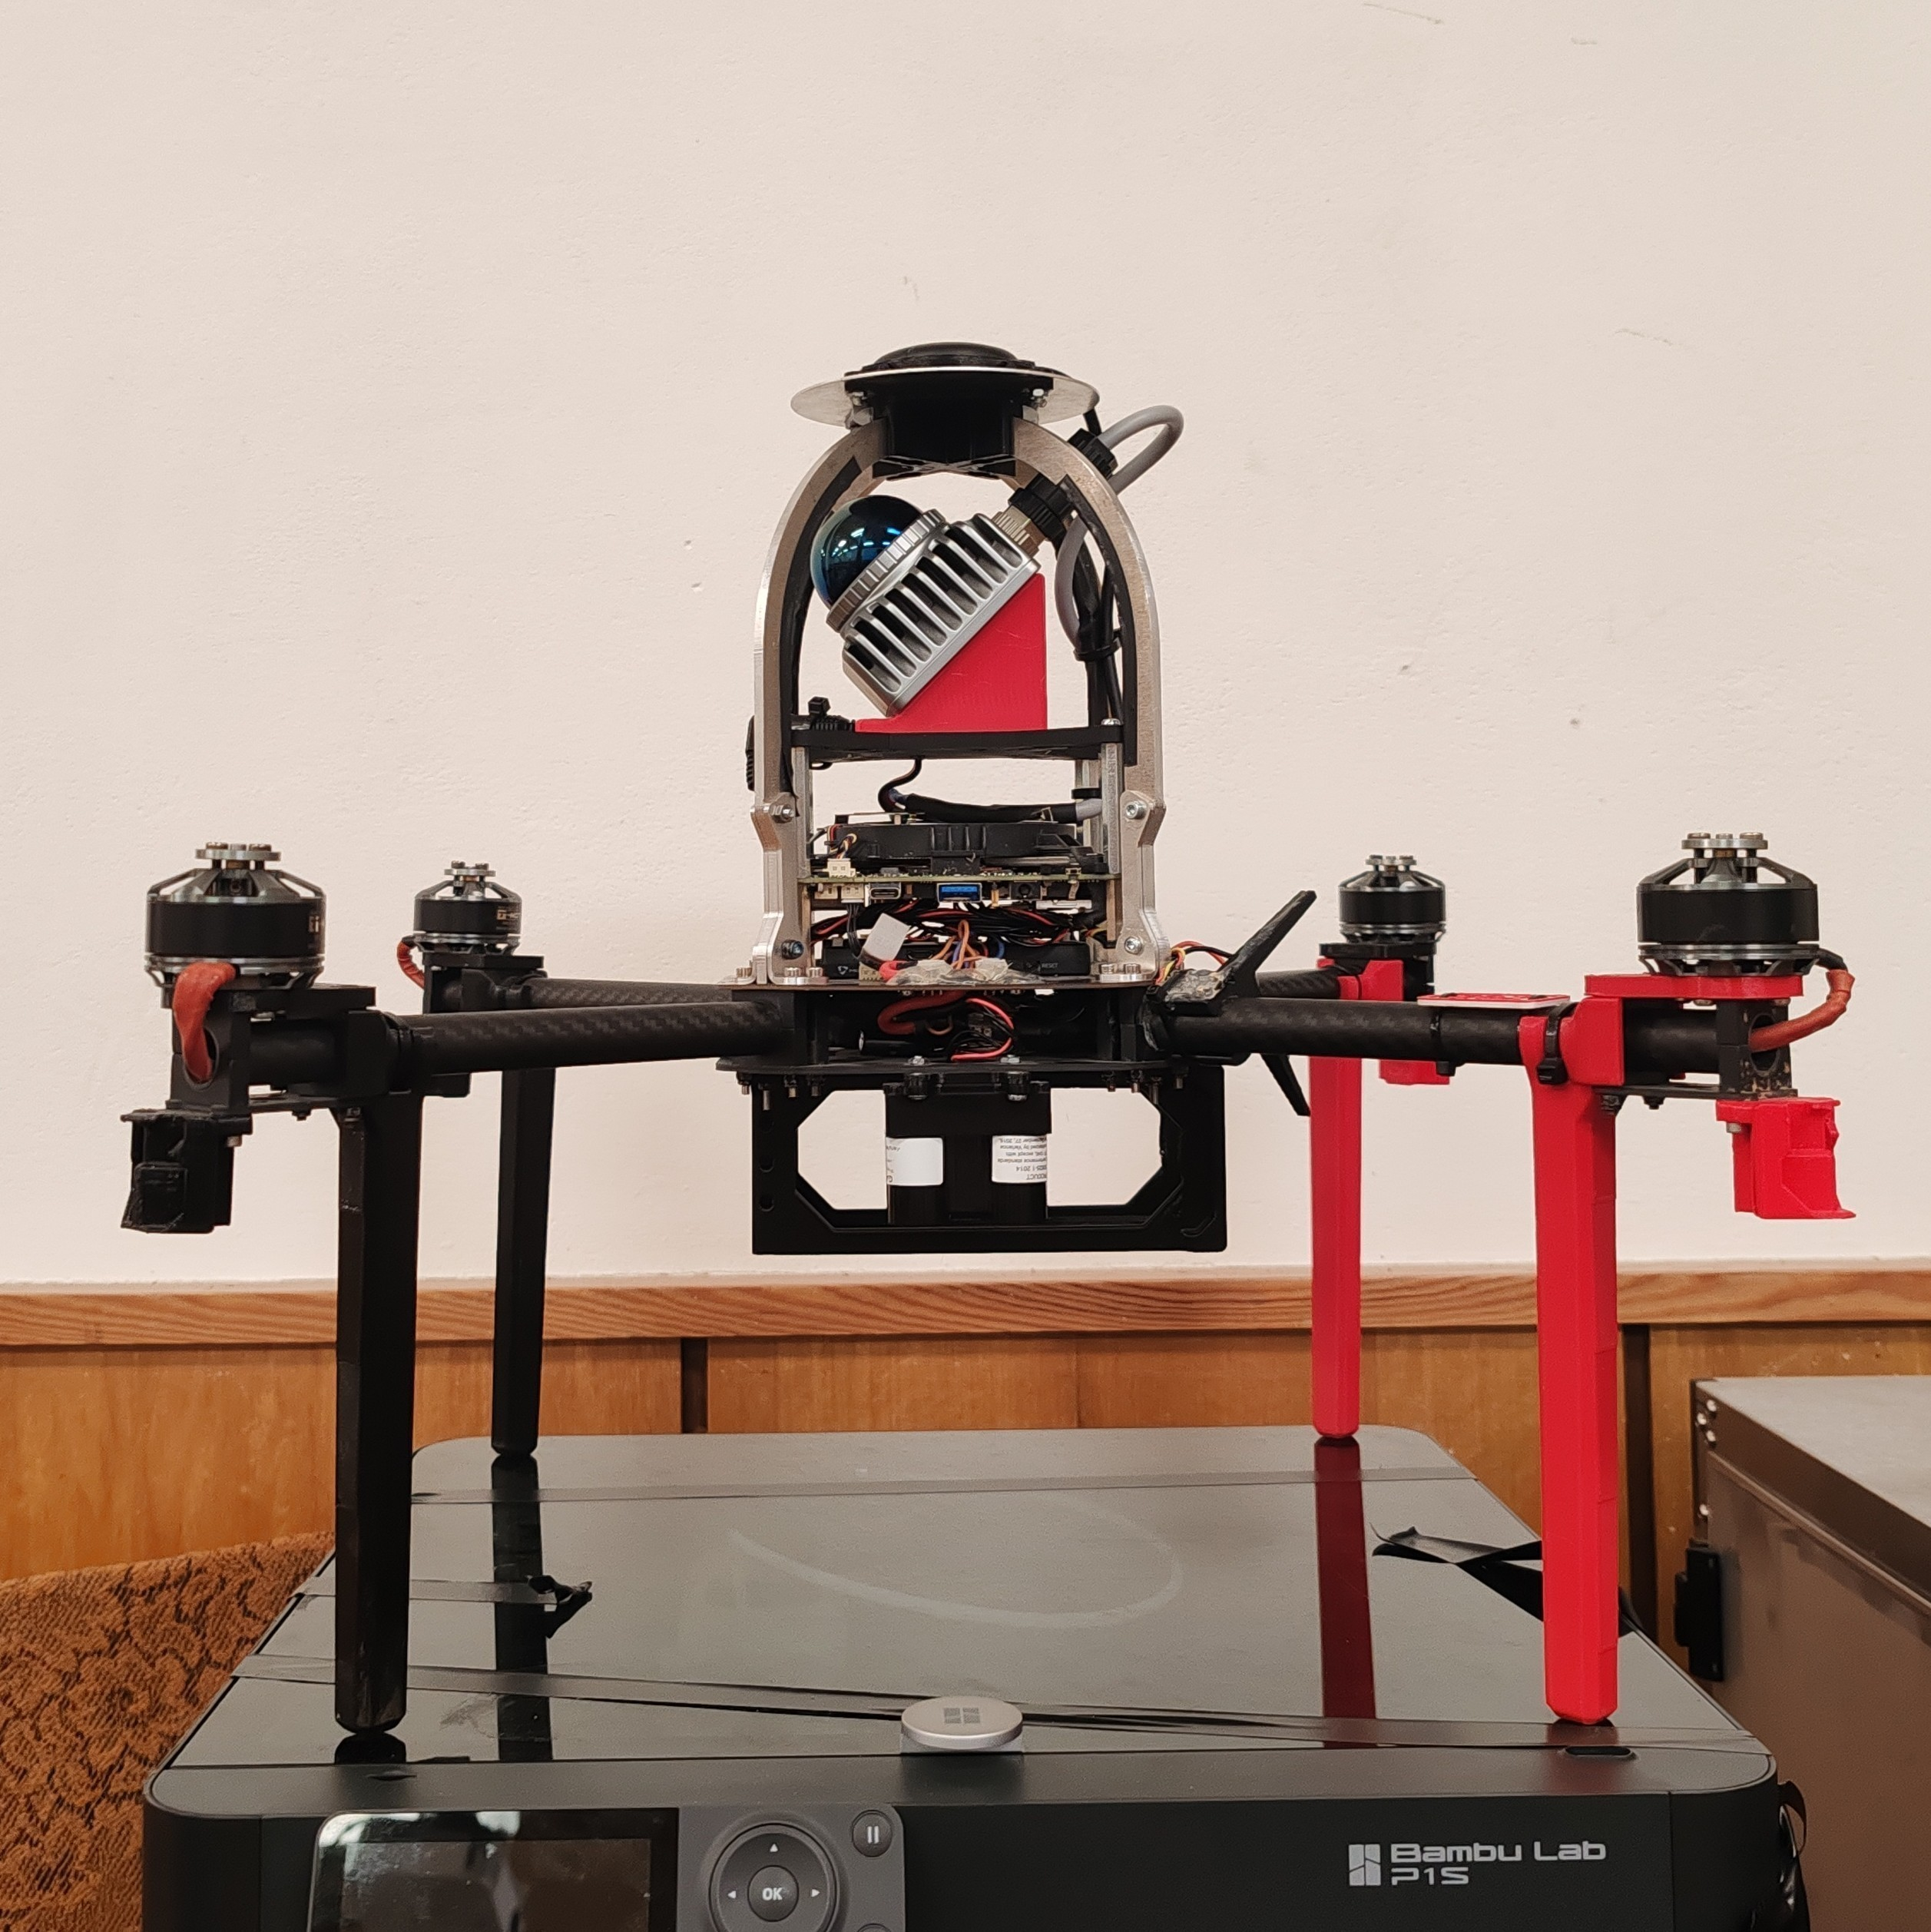
\includegraphics[width=0.48\textwidth]{./fig/photos/uav_photo.jpg}
                \label{fig:uav_1}
                }
                \caption{
                    UAV and \ac{LiDAR} mounting scheme.
                    Subfigure (a) shows a modeled UAV with visualized \ac{LiDAR} mounting parameters, including the \ac{LiDAR} elevation field of view $\alpha$ and tilt angle $\gamma$. 
                    Subfigure (b) displays the real UAV used in the experiment with the \ac{LiDAR} mounted according to the same configuration.                                                
                }
                \label{fig:uavs}
            \end{figure}


            In addition to the \ac{LiDAR} mounting angle, a software modification is implemented to account fo the \ac{LiDAR}'s limited \ac{FOV}.
            The algorithm uses map to partition cell $\mathcal{S}$ into cell $\mathcal{A}$, from which the centroid is computed to guide \ac{UAV} movement.
            To ensure safety, \ac{UAV} should only move only within their visible \ac{FOV}. 
            However, map information from areas outside the current \ac{FOV} can still be valuable. 

            Therefore, a constraint is intorduced - the \ac{UAV} maintains its yaw rotation towards the current centroid $\mathbf{c}_{\mathbf{A}}$ and moves towards it only if the centroid lies within a defined angular range in fron of the \ac{UAV}.

            To incorporate the \ac{LiDAR}'s \ac{FOV} into cell $\mathcal{S}$, two planes are defined based on the \ac{LiDAR}'s mounting configuration and vertical \ac{FOV}.
            Let $\mathbf{e}_z$ be unit vector alog the z-axis, $R_{off} \in SO(3)$ the offset rotation, and $R_{rpy} \in SO(3)$ the roll-pitch-yaw rotation.
            The normal vectors, $\mathbf{n}_1$ and $\mathbf{n}_2$ defining two planes are given by:
            \begin{equation}
                \mathbf{n}_1 = R_{rpy} \cdot R_{y}(\gamma) \cdot \mathbf{e}_z    
            \end{equation}
            \begin{equation}
                \mathbf{n}_2 = R_{rpy} \cdot R_{y}(\gamma - \alpha) \cdot \mathbf{e}_z    
            \end{equation}
            where $\alpha$ is the \ac{LiDAR}'s \ac{FOV} and $\gamma$ is the the mounting angle of the \ac{LiDAR}.

            Cell $\mathcal{S}$ is then modified by excluding points that lie outside the \ac{LiDAR}'s \ac{FOV}, defined by these two planes: 

            \begin{equation}
                \mathcal{S}_i' = \{ \mathbf{q} \in \mathcal{S}_i \mid \mathbf{n}1 \cdot (\mathbf{q} - \mathbf{p}_{LiDAR}) \geq 0 \land \mathbf{n}2 \cdot (\mathbf{q} - \mathbf{p}_{LiDAR}) \leq 0 \}
            \end{equation}
            where $\mathcal{S}_i'$ is the modified cell $\mathcal{S}$ and $\mathbf{p}_{LiDAR}$ is the exact position of the LiDAR sensor.

            This modification effectively restricts the points considered in the calculation of the centroid to only those within the \ac{LiDAR}'s \ac{FOV}.

            To incorporate map information from the surrounding area outside of the \ac{LiDAR}'s current \ac{FOV}, the following procedure is used.
            Firstly, both cells $\mathcal{S}_i$ and $\mathcal{S}_i'$ are created. These cells are partitioned into cells $\mathcal{A}_i$ and $\mathcal{A}_i'$ using voxels. 
            Cell $\mathcal{A}_i'$ is partitioned using voxels taht are actively sensed, while cell $\mathcal{A}_i$ is partitioned using the voxels from the whole surrounding.

            If the centroid computed from cell $\mathcal{A}_i$, $\mathbf{c}_{\mathcal{A}_i}$, is within the cell $\mathcal{A}_i'$, the \ac{UAV} is commanded to move towards $\mathbf{c}_{\mathcal{A}_i}$ while simu rotating its yaw towards it.
            However, if $\mathbf{c}_{\mathcal{A}_i}$ lies outside cell $\mathcal{A}_i'$, it is projected onto the closest point on the boundary of cell $\mathcal{A}_i'$.
            As the \ac{UAV} only moves if the centroid is within a certain angle in front of it, this projection onto the boundary of $\mathcal{A}_i'$ ensures that the \ac{UAV} primarily rotates towards the centroid until the centorid is within an angle in front of the \ac{UAV}.

            This procedure effectively utilizes the information fro mthe map while ensuring that the \ac{UAV} moves only within its actively sensed \ac{FOV}.

            \begin{figure}[H]
                \centering
                \subfloat[Visualization of planes defining cell $\mathcal{S}_i'$] {
                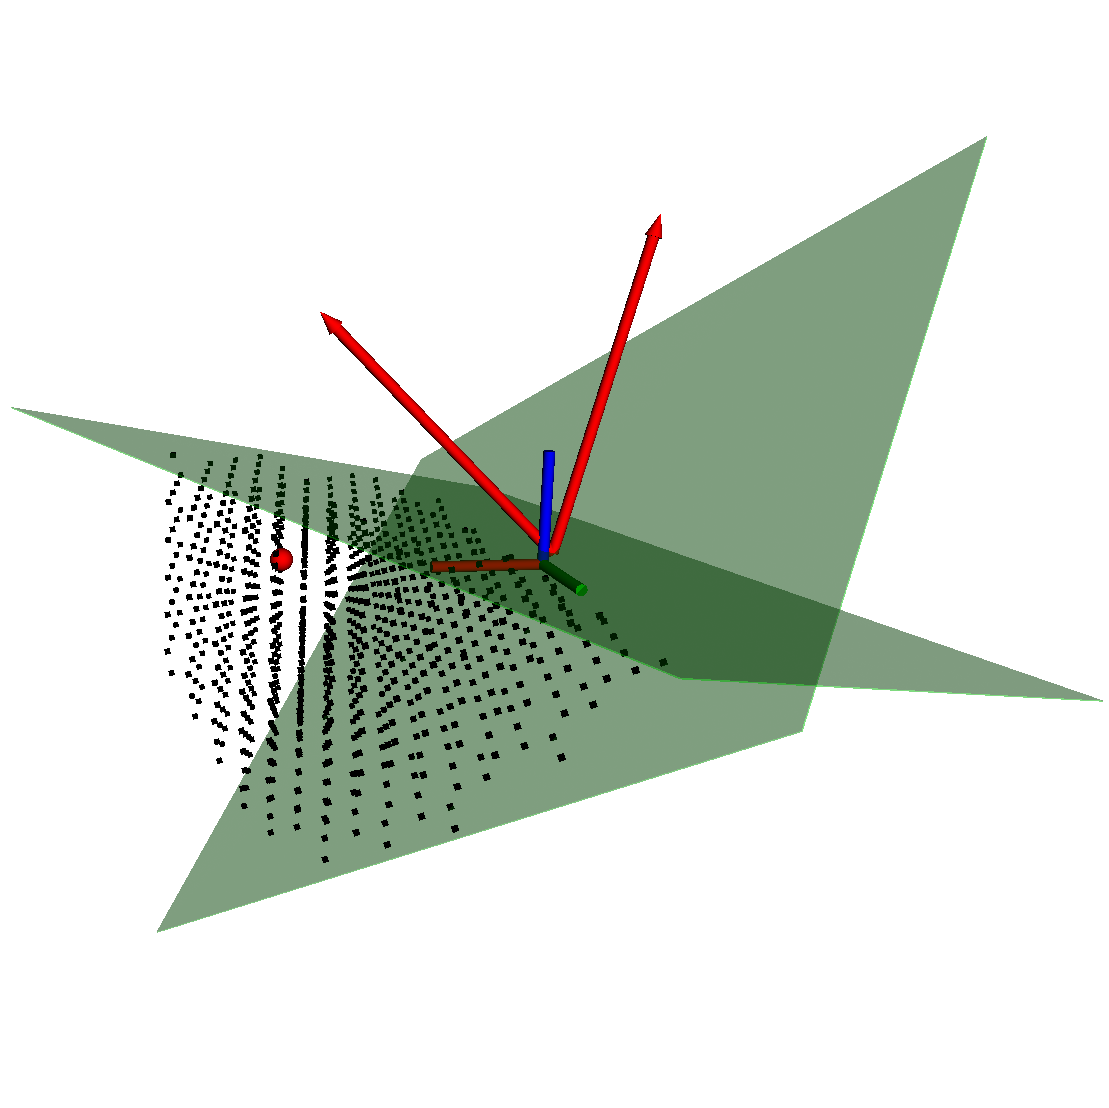
\includegraphics[width=0.48\textwidth]{./fig/rviz/cell_a_sliced_with_planes.png}
                \label{fig:cell_a_sliced_with_planes}
                }
                \caption{
                    RViz visualization of LiDAR field-of-view (FOV) planes. The UAV is represented by the XYZ coordinate axes. 
                    The green squares represent the two planes, defined by normal vectors $\mathbf{n}_1$ and $\mathbf{n}_2$, used to slice cell $\mathcal{S}_i$ and determine the modified cell $\mathcal{S}_i'$.
                    The red sphere represents the centroid $\mathbf{c}_{\mathcal{A}_i}$.
                }
                \label{fig:cell_a_sliced}
            \end{figure}

            % Apart from the mounting \ac{LiDAR} at an angle also software modificaiton is implemented. 
            % Right now a map is being used to partition cell S to cell A from that is computed centorid a there the uav progressees. 
            % For safety the UAV needs to move only where it sees, but the information from the map, where the uav does not see now, but this information can still be used. 
            % There fore this is introduced: UAV always sets it yaw rotation towards the current centroid $c_{\mathcal{A}}$ and moves towards it only if if the centroid is in front of the uav - there is an angle defined where the uav will move and where it will just keep rotating. 
            % So to utilize the map to have sense of what is behind the uav the 


            % For modification of cell S 2 planes are defined using real knowledge of how \ac{LiDAR} is mounted on the uav and livox vertical fov
            % Let $\mathbf{e}_z = \begin{bmatrix} 0 \\ 0 \\ 1 \end{bmatrix}$ be the unit vector along the z-axis,  
            % $R_{\text{off}} \in SO(3)$ the offset rotation, and  
            % $R_{\text{rpy}} \in SO(3)$ the roll-pitch-yaw rotation. 
            % $\alpha_1$, $\alpha_2$, $\alpha_3$

            % Then the resulting vector is given by:  
            % \[
            % \mathbf{n} = R_{\text{rpy}} \cdot R_{\text{off}} \cdot \mathbf{e}_z
            % \]

            % Modified cell S by slicing the cell S with this funciton:
            
            % \begin{equation}
            %     \mathcal{S}_i = {} 
            % \end{equation}
            % livox - 360 * 60 deg - account for centroid calculation
    
    \section{Experimental Results}
        This section presents the findings from both simulated and real-world experiments conducted to evaluate the proposed approach.
        \subsection{Simulation Setup}
            In the simulations, a virtual forest environment was created. 
            Initially, a raycasting approach from the UAV to the simulated trees was considered for obstacle detection. 
            However, due to its computational cost, a static point cloud representation of the entire forest was generated and published instead. 
            The forest was modeled as a collection of trees, with trunks represented by cylinders and crowns by spheres.

            The forest was contained within a rectangular area defined by the following boundaries:
            \begin{itemize}
                \item $x_{min}$ = -20.0 m
                \item $x_{max}$ =  20.0 m
                \item $y_{min}$ = -32.0 m
                \item $y_{max}$ =  32.0 m
            \end{itemize}
            A total of 100 trees were randomly generated within this area, with a minimum separation distance of 3 meters between them. 
            The trees were generated with the following parameter variances:
            \begin{itemize}
                \item Trunk radius: 0.5 $\pm$ 0.2 m
                \item Tree height: 7.5 $\pm$ 2.0 m
                \item Crown radius: 2.5 $\pm$ 0.5 m
            \end{itemize}
            The UAV's starting position was set at one corner of the rectangular area (-22.0, -33.0, 2.0), and the goal position was set at the opposite corner (22.0, 33.0, 5.0), resulting in an approximate distance of 80 meters between them.

            It is important to note that the right-hand rule and z rule, described in the previous chapter, are not required for effective coordination in this static forest environment.
            Also, the point-lio estimator and Bonxai mapping were not simulated.

            The specific values of the parameters used in the experiments are summarized in following table \ref{tab:rbl_forest_simulation_parameters}:
            \begin{table}[H]
                \centering
                \caption{Parameters Used in Experiments}
                \begin{tabular}{|l|l|}
                    \hline
                    Parameter & Value \\
                    \hline
                    \hline
                    Sensing radius ($r_s$) & 3.5 m \\ \hline
                    Update rate & 10 Hz \\ \hline
                    Encumbrance & 0.5 m \\ \hline
                    $d_1 = d_3 = d_5$ & 0.5 m \\ \hline
                    $d_2 = d_4 = d_6$ & 1.0 m \\ \hline
                    $\beta_i^D$ & 0.5  \\ \hline
                    $\eta$ & 0.9  \\ \hline
                \end{tabular}
                \label{tab:rbl_forest_simulation_parameters}
            \end{table}
            
            The UAV dynamics are the same as described in the previous chapter and detailed in Table \ref{tab:uav_constraints}. 
            Each simulation was run 10 times.            

        \subsection{Performance in Simulated Environments}
            The simulation results highlight the proposed solution capability in navigating inside dense forest environments. 
            The UAV demonstrated effective obstacle avoidance, reacting appropriately to simulated trees while maintaining efficient trajectory without unnecessary detours.
            Convergence towards the designated goal waypoint was consistently achieved in a stable manner.

            \begin{table}[H]
                \centering
                \renewcommand{\arraystretch}{1.2}
                \begin{tabular}{|l|c|c|c|c|}
                \hline
                                                  & \( SR \ [\%] \) & \( \overline{L} \ [\mathrm{m}] \) & \( \overline{t} \ [\mathrm{s}] \) &  \( \overline{v} \ [\mathrm{m/s}] \)     \\ \hline
                Simulation through forest 10 time & 100.00          & 91.99 $\pm$ 0.96                  & 150.89 $\pm$ 0.88                  &  0.85 $\pm$ 0.00                         \\ \hline
                \end{tabular}
            \end{table}

            \begin{figure}[H]
                \centering
                \subfloat[] {
                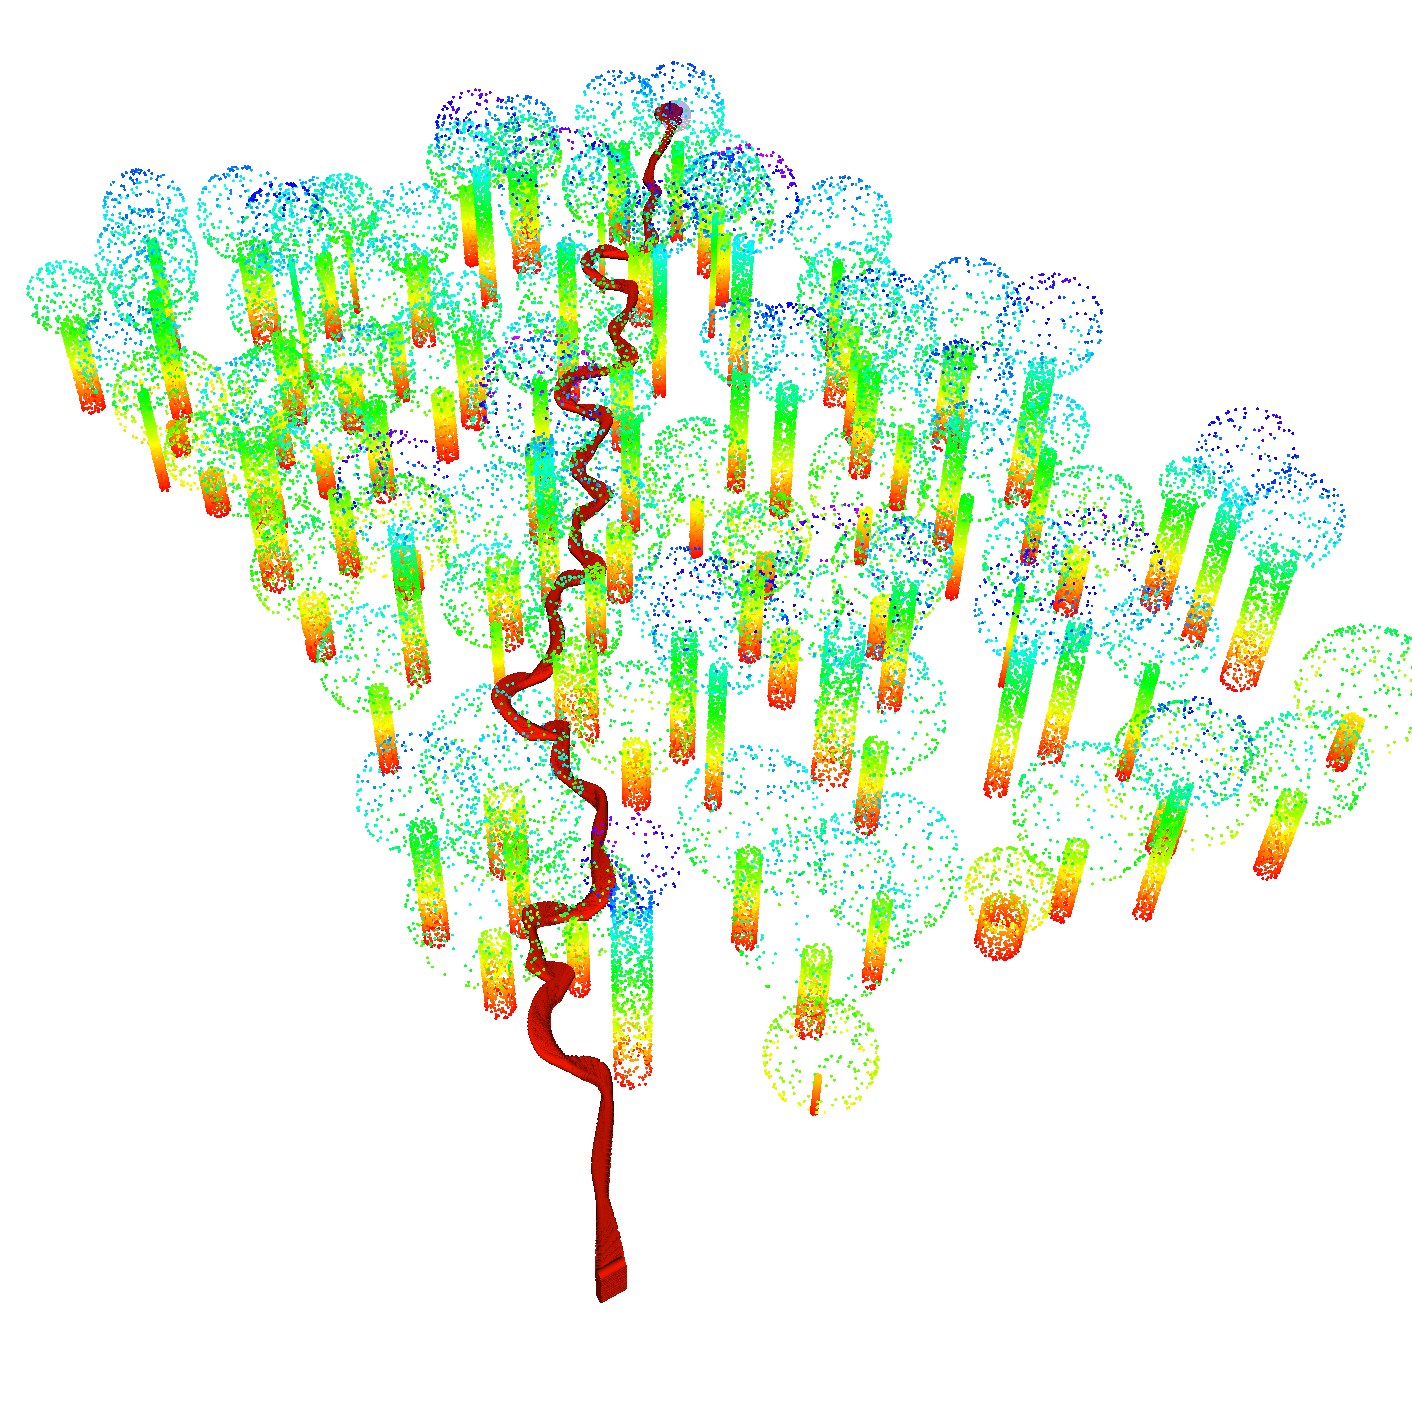
\includegraphics[width=0.48\textwidth]{./fig/rviz/simulation_forest.png}
                \label{fig:simulated_forest}
                }
                \caption{
                    visualization of simulated forest and path the uav took (red line)
                }
                \label{fig:simulated_forest_path}
            \end{figure}

        \subsection{Real-World Experiments in a Forest Environment}
            Following the successful simulation validation, the \ac{RBL} algorithm was tested through real-world experiments conducted in a forest environment.
            \begin{itemize}
                \item \textbf{Location: } \\
                    The chosen forest site presented a relatively clear environment, considered 'friendly' for initial UAV flight tests. 
                    To increase the navigational challenge and better test the obstacle avoidance capabilities, additional branches were placed near trees within the flight area after a few successfull flights. 
                    The point cloud filtration parameters were set to discard points closer than 1.0 meter (to avoid detecting the \ac{UAV}'s own propellers) and farther than 40 meters.
                \item \textbf{UAV Platform: } \\
                    A custom-built multirotor UAV from the MRS group was used for this experiment (TODO ask for specifications). 
                    It was equipped with a primaryly with LiDAR mounted on top for environmental perception and state estimation.
                    While other sensors like GPS (unreliable in the forest), a Garmin altimeter, and a barometer were present on the platform, they were not directly used by the \ac{UAV}.
                \item \textbf{Experimental Procedure: } \\
                    Each experimental run followed a defined procedure. 
                    First, the necessary software components were launched within a tmux session on the ground. 
                    A safety pilot then armed the UAV and performed a manual takeoff to a safe altitude. 
                    Once airborne and stable, the \ac{RBL} algorithm was initiated, commanding the UAV towards a predefined goal. 
                    The flight was continuously monitored via visualization in Rviz and observing the \ac{UAV}. 
                    If the UAV approached an obstacle too closely or exhibited unsafe behavior, the safety pilot immediately terminated the autonomous mode, took manual control, and landed the UAV. 
                    Between runs, key algorithm parameters, such as those controlling navigation 'aggressivity' (e.g., the scale of cells in the RBL and the weighting function used for path planning), were adjusted based on observations from the previous flight, and the experiment was repeated.
                \item \textbf{Safety Measures: } \\
                    Safety was paramount throughout the experiments. 
                    A trained safety pilot maintained visual line-of-sight with the UAV at all times and was prepared to immediately take manual control via the remote controller should any unsafe condition arise.
                \item \textbf{Data Collected: } \\
                    For safety reasons, data logging was initiated only after the manual takeoff was complete. 
                    During the autonomous flight part and subsequent landing, all relevant ROS topics (including sensor data, estimated state, \ac{RBL} cells, centroid) were recorded into rosbag files for detailed post-flight analysis.
                \item \textbf{Challenges Encountered: } \\
                    Several challenges emerged during real-world deployment. 
                    A significant set-back involved correctly managing coordinate frame transformations, particularly due to the slight tilt of the top-mounted LiDAR sensor. 
                    Ensuring accurate alignment between the LiDAR's point cloud data, the Point-LIO state estimator, and the navigation algorithm's reference frame required careful configuration. 
                    Another challenge, which warrants further investigation (discussed in Future Work), related to the Bonxai mapping part. 
                    Occasionally, the mapper would map dynamic objects, such as leaves disturbed by propellers, into the static map. 
                    Due to the mapping algorithm's configuration, which was set to be conservative about removing potentially static obstacles to ensure safety, these incorrectly mapped 'ghost' obstacles were sometimes not removed even when subsequent scans showed they were no longer present. 
                    In some instances, this led to the UAV perceiving itself as surrounded by obstacles (effectively 'locking' itself), requiring the safety pilot to intervene and land.
            \end{itemize}

            \begin{figure}[H]
                \centering
                \subfloat[] {
                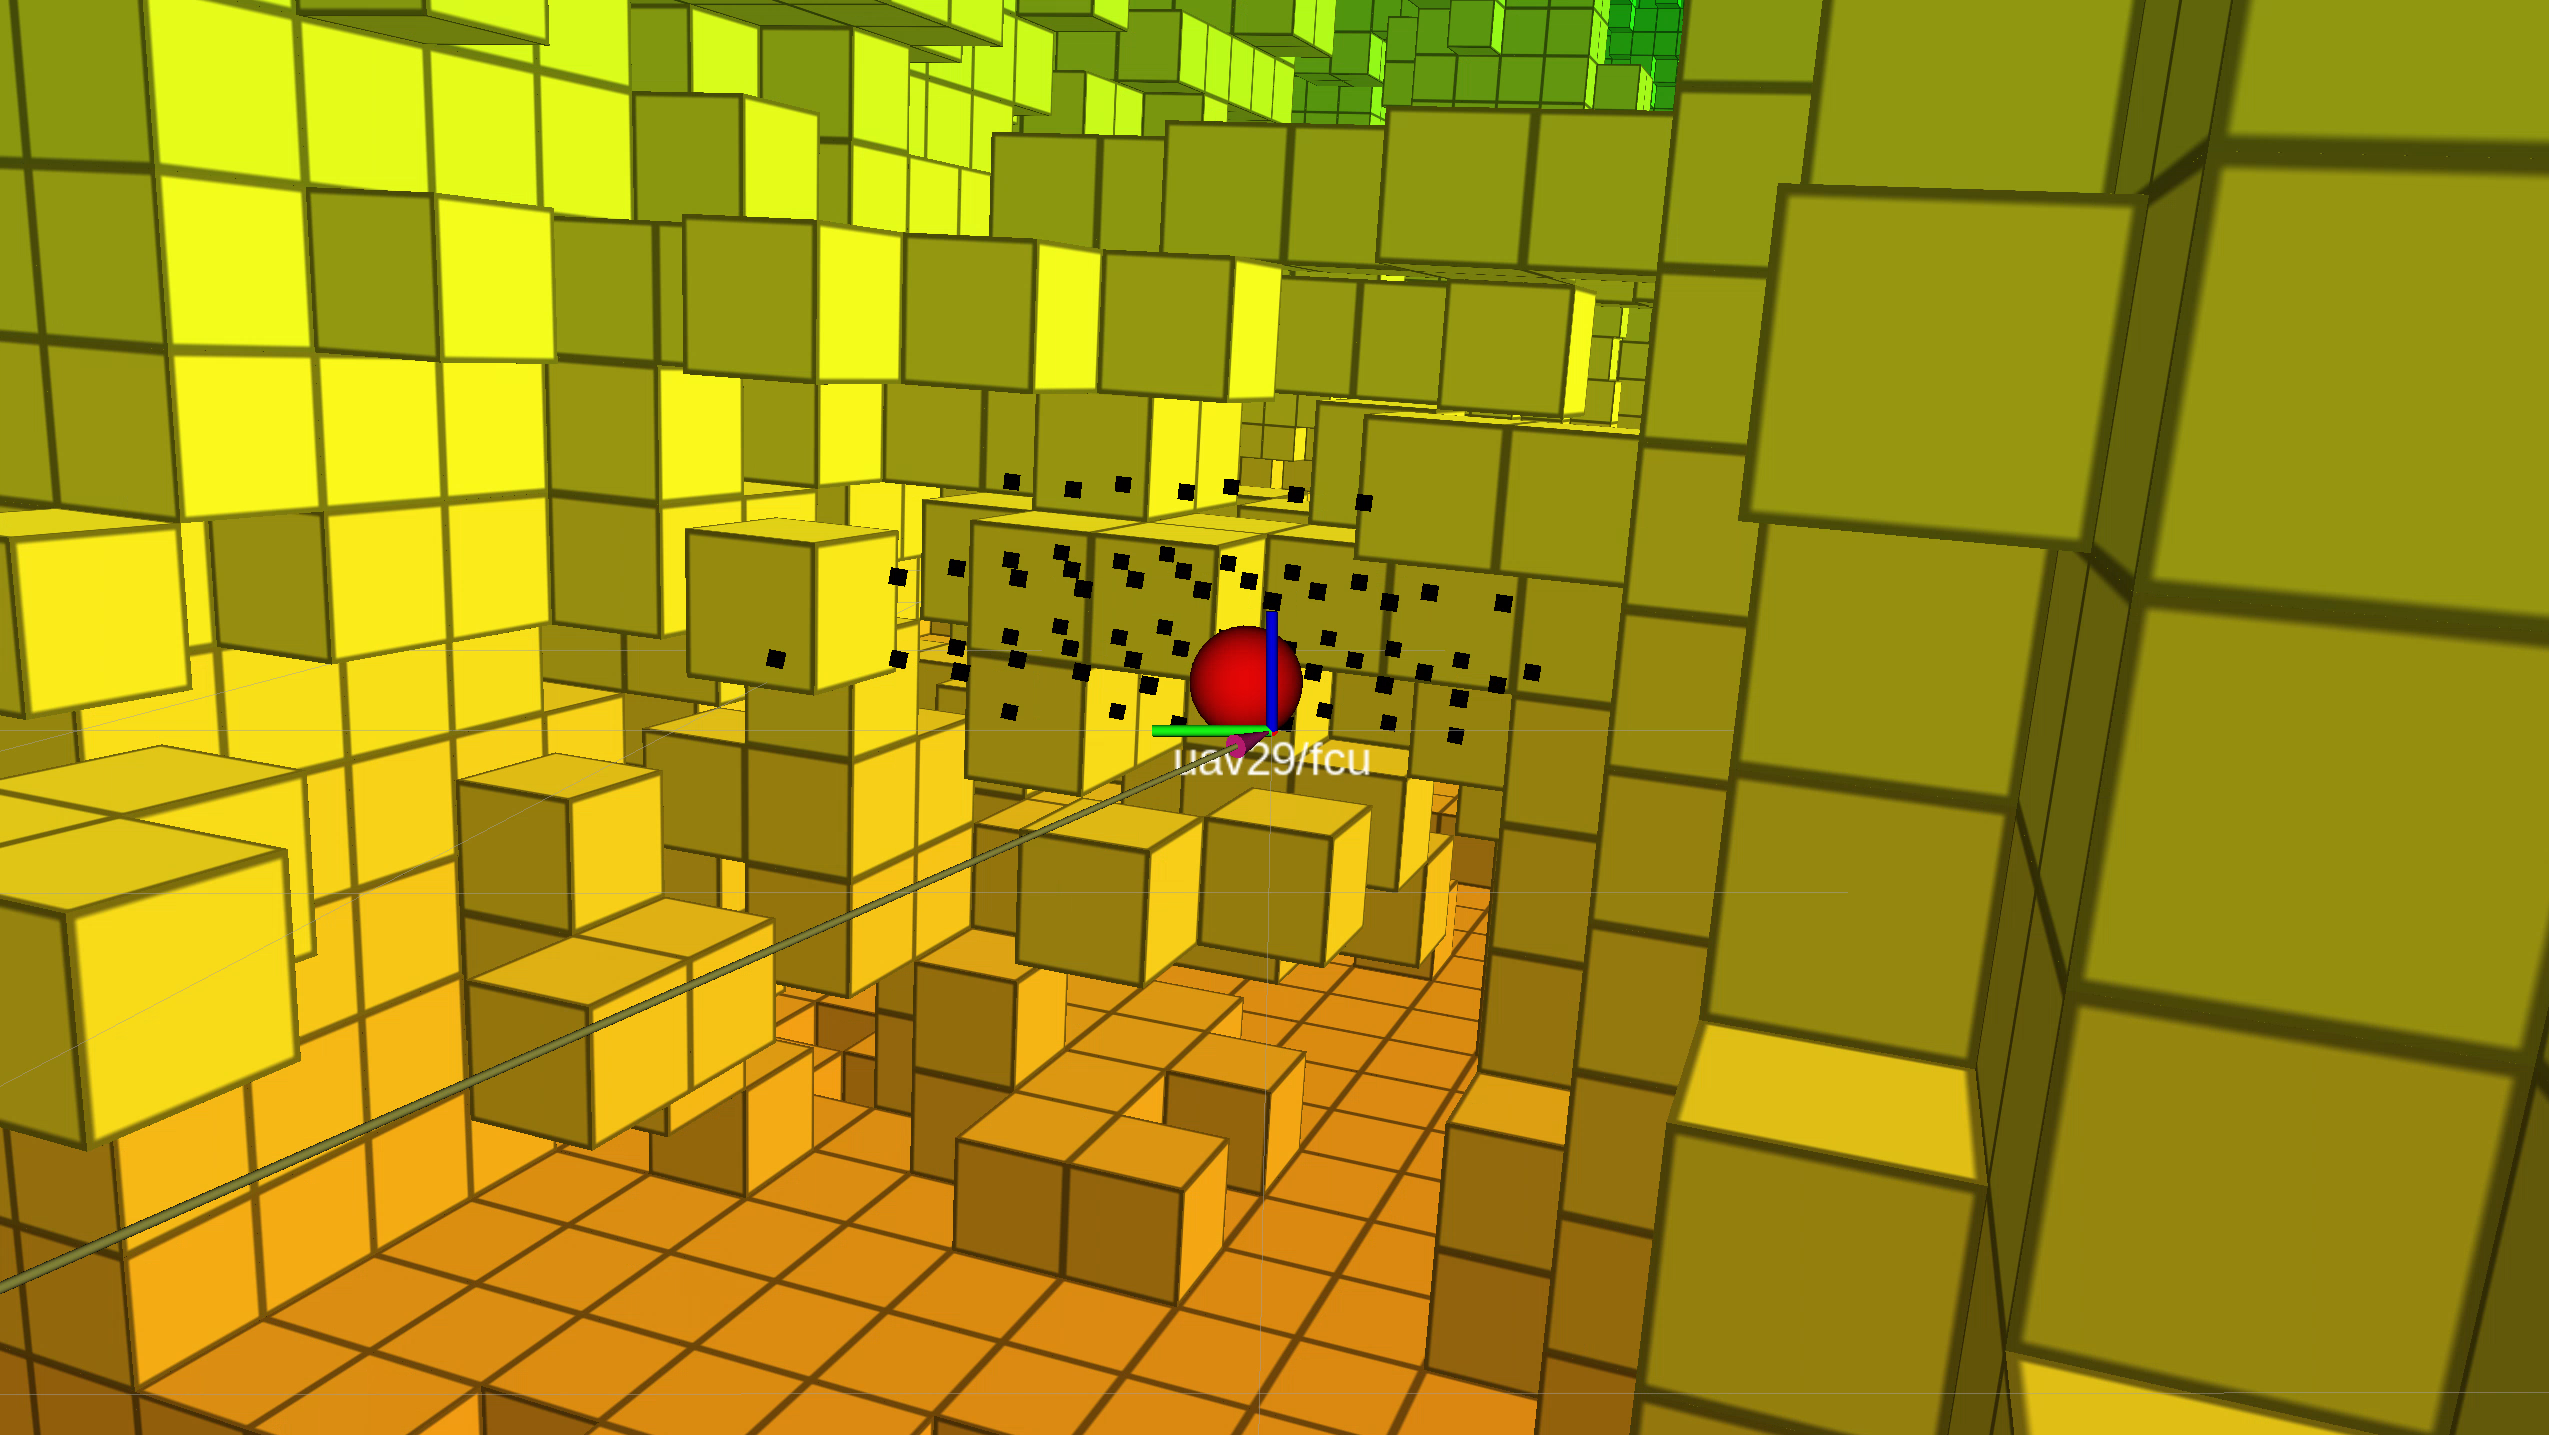
\includegraphics[width=0.48\textwidth]{./fig/rviz/deadlock_moment_mapping.png}
                \label{fig:map_fail_rviz}
                }
                \caption{
                    Visualization of a moment where the UAV incorrectly mapped leaves as obstacles directly in its path.
                }
                \label{fig:map_fail}
            \end{figure}

        
        \subsection{Performance in Real-World Experiment}
        * Metrics: Report the same metrics as in the simulation experiments where possible.

        \subsection{Comparative Analysis}
            * Simulation vs. Real-World Performance: Compare the results obtained in simulation with those from the real-world experiments.  Discuss any discrepancies and their possible causes.
            * Algorithm Performance: Compare your algorithm's performance with any existing algorithms or baseline methods.
            * Discussion of Limitations: Acknowledge any limitations of your algorithm or the experimental setup.
            * Future Work: Suggest potential areas for future research or improvements to the algorithm.
    
    \section{Conclusion}
        TODO
        Summary of contributions and some directions for future research
    








        % \subsection{Surface Reconstruction and Triangulation}
        %     The map has been used for surface reconstruction:
        %     To obtain a continuous surface representation from the point cloud, normal estimation and triangulation are performed. 
        %     This process involves estimating surface normals, combining them with point positions, and applying a triangulation algorithm to generate a polygonal mesh.
        %     \begin{itemize}
        %         \item \textbf{Normal Estimation: } \\ 
        %         Surface normals are estimated using the Point Cloud Library (PCL) TODOcite. 
        %         A k-d tree is employed to efficiently find neighboring points, and the normal at each point is computed based on its local neighborhood. 
        %         This provides information about the surface curvature and orientation.
        %         \item \textbf{Point Cloud and Normal Merging: } \\ 
        %         Once the normals are estimated, they are combined with the original point cloud to create a representation that includes both spatial position and surface orientation.
        %         \item \textbf{Triangulation Using Greedy Projection: } \\
        %         The point cloud is converted into a polygonal mesh using the Greedy Projection Triangulation (GP3) method. 
        %         This algorithm forms triangles between neighboring points while enforcing constraints on edge length, surface angles, and normal consistency. 
        %         A k-d tree is used to accelerate the search for nearest neighbors, ensuring efficient mesh generation.
        %         \item \textbf{Results: } \\ 
        %         The output is a polygonal mesh that approximates the underlying surface of the point cloud. 
        %         This mesh can be used for visualization and obstacle avoidance.
        %     \end{itemize}
        %     This has been tried, but turned out to be unnecessary computationally expensive and on the UAV onboard computer slow. 
        %     It was able to approximate surface of its surrounding semi-well. 
        %     But due for it being slow a simplier method have been used - (Directly using voxels to modify cell A) instead of aporximating surface.
        %     So I just wanted to quiky say that this was tested, unsuccesflully so no future development of this methos is recomended or something like that. 


        %     There will be picture from rviz how it approximated surface.
